%
% teil1.tex -- Beispiel-File für das Paper
%
% (c) 2020 Prof Dr Andreas Müller, Hochschule Rapperswil
%
\section{Spiegelung}
\rhead{Spiegelung}

Die Spiegelung ist eine grundlegende, geometrische Operation, aus welcher man weitere Operationen, wie beispielsweise die später beschriebene Rotation, ableiten kann. Da die geometrische Algebra für geometrische Anwendungen ausgelegt ist, sollte die Spiegelung auch eine einfache, praktische Formulierung besitzen.
\begin{figure}
	\centering
	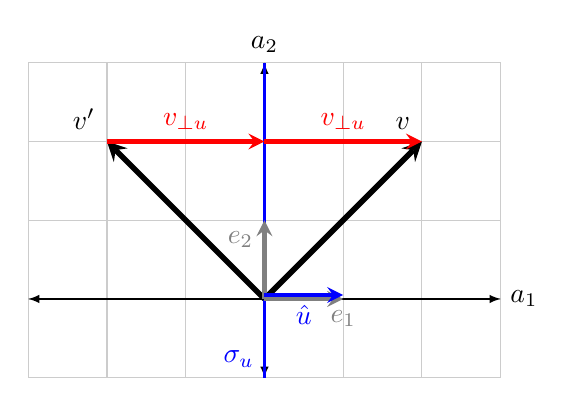
\begin{tikzpicture}[>=latex]
		\draw[thin,gray!40] (-3,-1) grid (3,3);
		\draw[<->] (-3,0)--(3,0) node[right]{$a_1$};
		\draw[<->] (0,-1)--(0,3) node[above]{$a_2$};
		\draw[blue, line width=1.0pt] (0,3)--(0,-1) node[anchor=south east]{$\sigma_u$};
		\draw[line width=2pt,black,-stealth](0,0)--(2,2) node[anchor=south east]{$\boldsymbol{v}$};
		\draw[line width=2pt,black,-stealth](0,0)--(-2,2) node[anchor=south east]{$\boldsymbol{v'}$};
		\draw[line width=1.5pt,gray,-stealth](0,0)--(1,0) node[anchor=north]{$\boldsymbol{e_1}$};
		\draw[line width=1.5pt,gray,-stealth](0,0)--(0,1) node[anchor=north east]{$\boldsymbol{e_2}$};
		\draw[line width=1.5pt,red,-stealth](0,2)--(2,2) node[xshift=-1cm, yshift=
		0.25cm]{$\boldsymbol{v_{\perp u}}$};
		\draw[line width=1.5pt,red,-stealth](-2,2)--(0,2) node[xshift=-1cm, yshift=
		0.25cm]{$\boldsymbol{v_{\perp u}}$};
		\draw[line width=1.5pt,blue,-stealth](0,0.05)--(1,0.05) node[xshift=-0.5cm, yshift=-0.25cm]{$\boldsymbol{\hat{u}}$};
	\end{tikzpicture}
	\caption{Spiegelung des Vektors $\mathbf{v}$ an der Spiegelebene $\sigma_u$ mit dem Normalenvektor $\mathbf{\hat{u}}$}
	\label{BildSpiegelung}
\end{figure}

\subsection{Linearen Algebra}
Aus der linearen Algebra ist bekannt, dass man eine Spiegelung an einer Ebene wie folgt beschreiben kann.
\begin{definition}
	Die Abbildung der Spiegelung in der linearen Algebra mit dem Normalenvektor $\mathbf{\hat{u}}$ zur Spiegelebene ist
	\begin{equation} \label{RefLinAlg}
		\mathbf{v} = \mathbf{v_{\perp u}} + \mathbf{v_{\parallel u}} \enspace\mapsto\enspace \mathbf{v'} =  \mathbf{v_{\perp u}} - \mathbf{v_{\parallel u}} = \mathbf{v} - 2 \cdot \mathbf{v_{\parallel u}}.
	\end{equation}
\end{definition}
Es scheint für diese Formel \eqref{RefLinAlg} aber umständlich zu sein, weitere Spiegelungen mit weiteren Spiegelebenen anzufügen. Weil man $\mathbf{v_{\parallel u}}$ auch als Skalarprodukt $\mathbf{v_{\parallel u}} = \mathbf{\hat{u}} \cdot \mathbf{v}$ schreiben kann, ist es leicht diese Abbildung auch als Matrix darzustellen. Sei $\mathbf{\hat{u}}$ ein Normalenvektor auf die Spiegelungsebene, also $\mathbf{\hat{u}}\perp \sigma_u$, und sei ausserdem normiert $|\mathbf{\hat{u}}| = 1$, dann kann man die Spiegelung durch die Matrix
\begin{align}
	S = E - 2\mathbf{\hat{u}\hat{u}}^t
\end{align}
beschrieben werden. In der zweiten und dritten Dimension ergibt die Berechnung
\begin{align} \label{Spiegelmatrizen}
	S_2 = \begin{pmatrix}
		1-2u_1^2 & -2u_1u_2 \\
		-2u_1u_2 & 1-2u_2^2
	\end{pmatrix}\enspace\text{und}\enspace
	S_3 = \begin{pmatrix}
		1-2u_1^2 & -2u_1u_2 & -2u_1u_3\\
		-2u_1u_2 & 1-2u_2^2 & -2u_2u_3\\
		-2u_1u_3 & -2u_2u_3 & 1-2u_3^2\\
	\end{pmatrix}.
\end{align}
Diese Spiegelmatrizen gehören der orthogonalen Matrizengruppe $S_n\in \text{O}(n)$ an. Die Matrizengruppe $\text{O}(n)$ haben die Eigenschaft $S_n^t S_n = E$, was bedeutet, dass die Länge und Winkel bei der Abbildung beibehalten bleiben. Zusätzlich sind die Spiegelmatrizen symmetrisch, es gilt $S_n^t = S_n$. Somit liefert zweimal dieselbe Spiegelung wieder die identische Abbildung, wie man aus
\begin{align}
	S_n^t S_n = S_n^2 = E
\end{align}
schliessen kann.

\subsection{Geometrische Algebra}
Wir definieren zuerst die Inverse eines Vektors, welche in dieser Form nicht in der linearen Algebra nicht existiert.
\begin{definition}
	Die Inverse eines Vektors wird definiert als
	\begin{align} \label{InverseGA}
		\mathbf{u}^{-1} = \dfrac{\mathbf{u}}{|\mathbf{u}|^2}. 
	\end{align}
\end{definition}
Diese Definition ist sinnvoll, da wegen $\mathbf{u}^2 = |\mathbf{u}|^2$ folgt
\begin{align}
	\mathbf{uu}^{-1} = \mathbf{u} \frac{\mathbf{u}}{|\mathbf{u}|^2} = \frac{\mathbf{u}^2}{|\mathbf{u}|^2} = \frac{|\mathbf{u}|^2}{|\mathbf{u}|^2} = 1.
\end{align}
Der Vektor $\mathbf{u}^{-1}$ in \eqref{InverseGA} ist also tatsächlich das inverse Element im Sinne des Produktes in der geometrischen Algebra.
Die geometrische Algebra leitet aus der obigen Formel \eqref{RefLinAlg} für eine Spiegelung eine einfache und intuitive Form her, welche auch für weitere Operationen erweitert werden kann.
\begin{definition}
	Die Abbildung der Spiegelung in der geometrischen Algebra mit dem senkrechten Vektor $\mathbf{u}$ zur Spiegelungsebene $\sigma_u$ ist 
	\begin{align}\label{RefGA}
		\mathbf{v} \enspace\mapsto\enspace \mathbf{v}' = -\mathbf{uvu}^{-1}
	\end{align}
\end{definition}
Diese Abbildung muss stimmen, weil man durch die Schlussfolgerungen \eqref{uperpv} und \eqref{uparallelv} die Zusammenhänge
\begin{align}
	\mathbf{uv_{\perp u}} = -\mathbf{v_{\perp u}u} \enspace\text{und}\enspace \mathbf{uv_{\parallel u}}=\mathbf{v_{\parallel u}u}
\end{align}
der geometrischen Produkte findet und somit die Abbildung aus der geometrischen Algebra \eqref{RefGA} wegen
\begin{align}
	\mathbf{v}' = -\mathbf{uvu}^{-1} = -\mathbf{uv_{\perp u}u}^{-1} - \mathbf{uv_{\parallel u}u}^{-1} = -(-\mathbf{v_{\perp u}}\underbrace{\mathbf{u})\mathbf{u}^{-1}}_{1} -(\mathbf{v_{\parallel u}}\underbrace{\mathbf{u})\mathbf{u}^{-1}}_{1} = \mathbf{v_{\perp u}} - \mathbf{v_{\parallel u}}
\end{align}
gleichbedeutend zu der Definition \eqref{RefLinAlg} der Spiegelung ist.

Verwendet man für $\mathbf{u}$ nur einen Einheitsvektor $\mathbf{\hat{u}}$, welcher die Länge 1 besitzt, wird die Gleichung \eqref{RefGA} zu
\begin{align}
	\mathbf{v'} = -\mathbf{\hat{u}v\hat{u}}
\end{align}
vereinfacht. Im Gegensatz zu den Abbildungen in der linearen Algebra, welche in jeder anderen Dimension, durch andere Matrizen \eqref{Spiegelmatrizen} beschrieben werden müssen, ist es in der geometrischen Algebra immer der gleiche Vorgehensweise. Zudem ist diese kompakte Schreibweise in der linearen Algebra nicht möglich, da bis auf das Vektorprodukt in der dritten Dimension keine Multiplikation von Vektoren definiert ist. 
